\documentclass[]{article}

\usepackage{mathtools}
\usepackage{listings}
\usepackage{clrscode}
\usepackage{algorithm}
\usepackage{algorithmic}
\usepackage{graphicx}
\usepackage[top=2cm, bottom=2cm, left=2cm, right=2cm]{geometry}
\DeclareMathOperator*{\argmin}{arg\,min}
\DeclareMathOperator*{\argmax}{arg\,max}

\title{Homework 1}
\date{2015-10-15}
\author{Jingwei Zhang 201528013229095}

\begin{document}
    \maketitle
    \section{Problem 1}
    \begin{figure}[H]
        \centering
        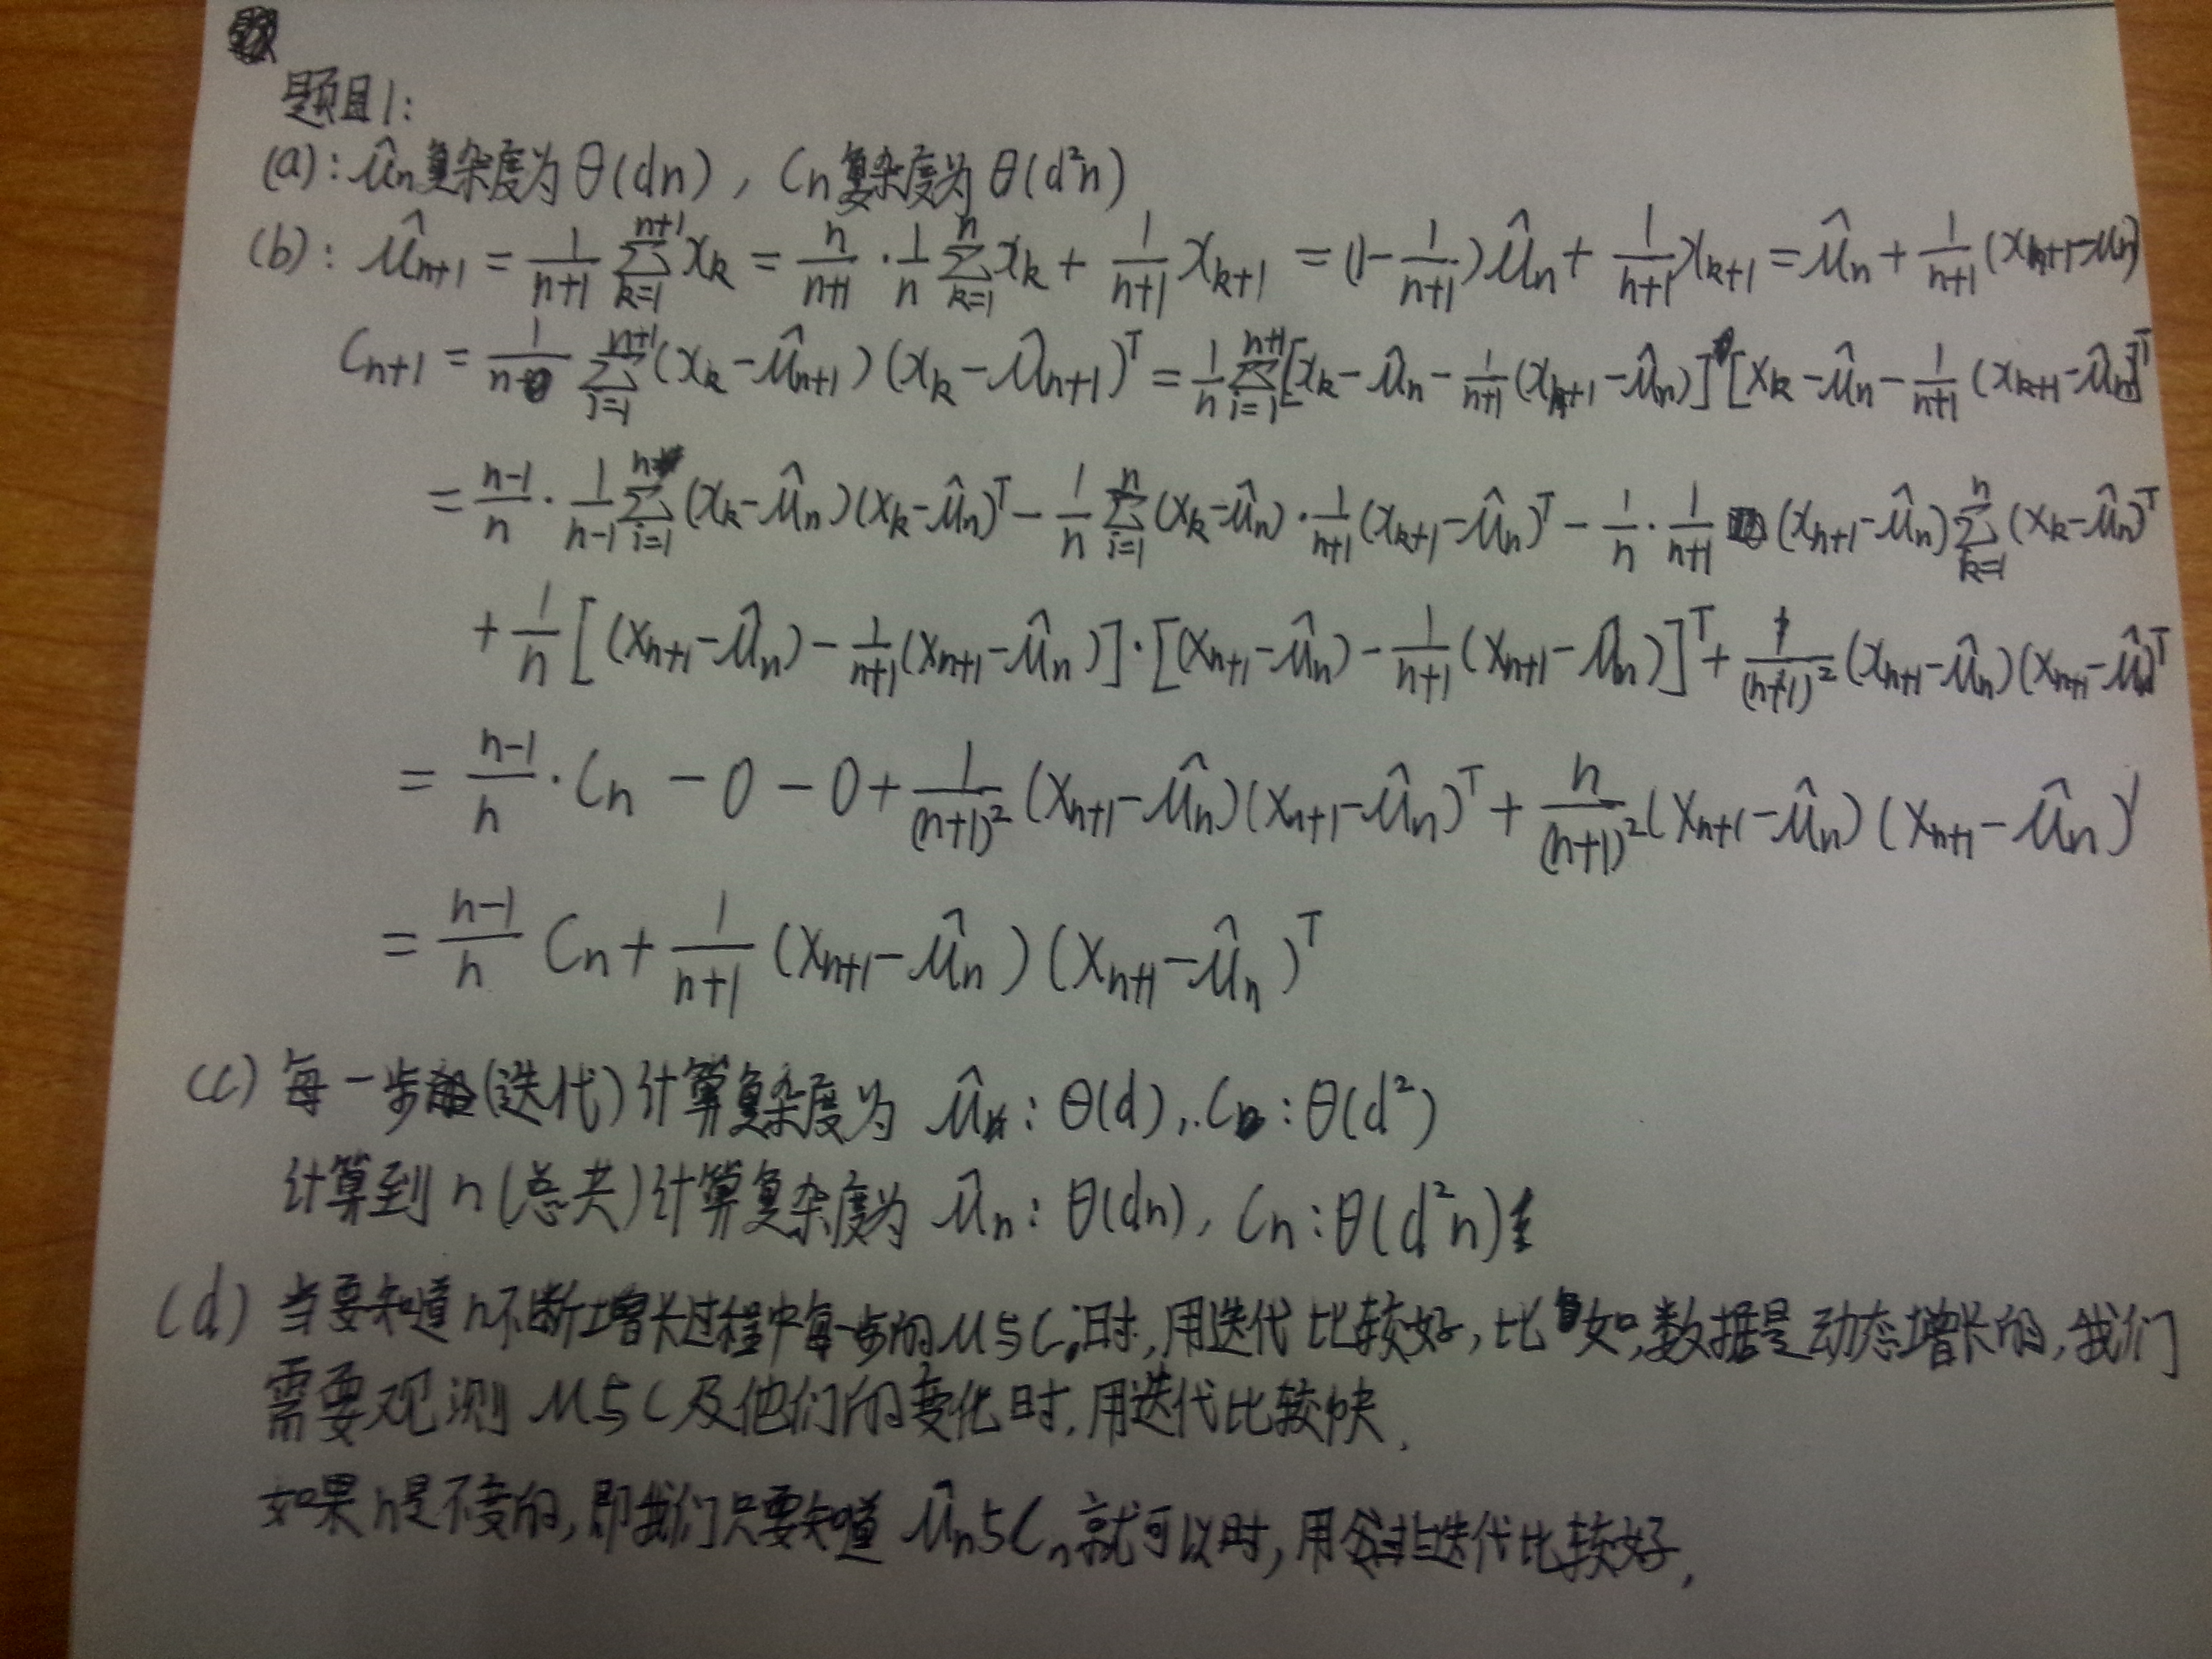
\includegraphics[scale=0.15]{P1.jpg}
    \end{figure}
    \section{Problem 2}
    \subsection{a}
According to the question , we have the data set $\mathcal{D} = \left\{ \left(\begin{aligned}1\\1\end{aligned}\right),\left(\begin{aligned}3\\3\end{aligned}\right),\left(\begin{aligned}2\\\star\end{aligned}\right)\right\}$, we have :
\begin{align*}
	Q(\theta, \theta^0) =& E_{x_{32}} \left[ \ln P(x_g,x_b;\theta)|\theta^0,\mathcal{D} \right]\\
	=& \int \limits_{- \infty}^{+ \infty} [\ln P(x_1 |\theta) +\ln P(x_2|\theta) + \ln P(x_3|\theta)]P(x_{32}|\theta^0,x_{31} = 2)dx_{32} \\
	=&\ln P(x_1 |\theta) +\ln P(x_2|\theta) +  \int \limits_{- \infty}^{+ \infty} \ln P(x_3|\theta)P(x_{32}|\theta^0,x_{31} = 2)dx_{32} \\
	=&\ln P(x_1|\theta)+\ln P(x_2|\theta)+2e\int \limits_{- \infty}^{+ \infty} \ln P\left[\left( \scriptstyle 2 \atop x_{32}\right)\right]P\left[ \left(\scriptstyle 2 \atop x_{32} \right) \big | \theta^0\right]dx_{32} 
\end{align*}
Then, let $T = 2e\int \limits_{- \infty}^{+ \infty} \ln P\left[\left( \scriptstyle 2 \atop x_{32}\right)\right]P\left[ \left(\scriptstyle 2 \atop x_{32} \right) \big | \theta^0\right]dx_{32}$, we have:
\paragraph{1.} If $3 \leq \theta_2 \leq 4$ :
\begin{align*}
	T =& \frac{1}{4} \int \limits_0^{\theta_2} \ln \left( \frac{1}{\theta_1} e^{-2\theta_1} \times \frac{1}{\theta_2}\right)dx_{32}\\
	=&\frac{1}{4} \theta_2 \ln \left( \frac{1}{\theta_1} e^{-2\theta_1} \times \frac{1}{\theta_2}\right)
\end{align*}
\paragraph{2.} If $4 < \theta_2 $ :
\begin{align*}
	T =& \frac{1}{4} \int \limits_0^4 \ln \left( \frac{1}{\theta_1} e^{-2\theta_1} \times \frac{1}{\theta_2}\right)dx_{32}\\
	=& \ln \left( \frac{1}{\theta_1} e^{-2\theta_1} \times \frac{1}{\theta_2}\right)
\end{align*}
\paragraph{3.} If $\theta < 3$ :
\begin{align*}
	T = 0
\end{align*}
Therefore,we get :
\begin{align*}
	Q(\theta,\theta^0) =& \ln P(x_1|\theta)+\ln P(x_2|\theta) + T \\
	=&-4\theta_1 - 2\ln (\theta_1 \theta_2) + T
\end{align*}
Because of :
\begin{align*}
	\int \limits_{-\infty}^{+\infty} P(x_1)dx_1 &= 1 \\
	\int \limits_{-\infty}^{+\infty} \frac{1}{\theta_1}e^{-\theta_1x_1}dx_1 &= 1
\end{align*}
Thus, above all we get the result :
\begin{align*}
	\theta_1 = 1
\end{align*}
\subsection{b}
\paragraph{(1)} $3 \leq \theta_2 \leq 4$,according to the formula of $Q(\theta,\theta^0)$,we get:
\begin{align*}
	Q(\theta,\theta^0) = -4 -\left(2\ln \theta_2 + \frac{1}{4} \theta_2(2+\ln \theta_2) \right)
\end{align*}
Therefore, when $\theta_2 = 3$ ,we get the max result,$Q(\theta,\theta^0) = -8.521$
\paragraph{(2)}$\theta_2 > 4$,according to the formula of $Q(\theta,\theta^0)$, we get:
\begin{align*}
	Q(\theta,\theta^0) = -6-3\ln \theta_2
\end{align*}
\paragraph{}Therefore, when $\theta_2 = 4$ ,we get the max result,$Q(\theta,\theta^0) = -10.159$
Thus , above all ,the result is $\theta = (3 \  \  \  4 )^t$.
    
    \section{Problem 3}
    \subsection{a}
    \begin{align*}
    \bar{p_n}(x) &= E[p_n(x)] \\
					&= \frac{1}{n h_n}\sum_{i=1}^n E \left[ \varphi\left(\frac{x-x_i}{h_n}\right)\right] \\
					&= \frac{1}{h_n} \int \varphi\left(\frac{x-v}{h_n}\right) p(v)dv\\
					&= \frac{1}{h_n} \int \frac{1}{\sqrt{2\pi}} \frac{1}{\sqrt{2\pi}\sigma} \exp\left[ -\frac{(x-v)^2}{2h_n^2} -\frac{(v-\mu)^2}{2\sigma^2}\right]dv \\
					&= \frac{1}{2\pi\sigma h_n} \exp\left[-\frac{1}{2}\left(\frac{x^2}{h_n^2}+\frac{\mu^2}{\sigma^2}\right)\right] \int \exp\left[-\frac{1}{2}\left(\frac{1}{h_n^2}+\frac{1}{\sigma^2}\right)v^2+\left(\frac{x}{h_n^2}+\frac{\mu}{\sigma^2}\right)v\right]dv \\
					&= \frac{\sigma'}{\sqrt{2\pi}h_n\sigma} \exp\left[-\frac{1}{2}\left(\frac{x^2}{h_n^2}+\frac{\mu^2}{\sigma^2}\right)+\frac{1}{2}\frac{\mu'^2}{\sigma'^2}\right] \int\frac{1}{\sqrt{2\pi}\sigma'}\exp\left[-\frac{1}{2}\left(\frac{v-\mu'}{\sigma'}\right)^2\right]dv \\
					&= \frac{\sigma'}{\sqrt{2\pi}h_n\sigma} \exp\left[-\frac{1}{2}\left(\frac{x^2}{h^2}+\frac{\mu^2}{\sigma^2}-\frac{\mu'^2}{\sigma'^2}\right)\right] \\
					&= \frac{1}{\sqrt{2\pi}h_n\sigma} \frac{h_n\sigma}{\sqrt{h_n^2+\sigma^2}} \exp\left[-\frac{1}{2}\left(\frac{x^2\sigma^2h_n^2+x^2\sigma^4+h_n^4\mu^2+h_n^2\mu^2\sigma^2}{h_n^2\sigma^2(h_n^2+\sigma^2)}-\frac{x^2\sigma^4+h_n^4\mu^2+2x\sigma^2h_n^2\mu}{h_n^2\sigma^2(h_n^2+\sigma^2)}\right)\right] \\
					&= \frac{1}{\sqrt{2\pi}} \frac{1}{\sqrt{h_n^2+\sigma^2}}	\exp\left[-\frac{1}{2}\frac{(x-\mu)^2}{h_n^2+\sigma^2}\right]
    \end{align*}
    \begin{align*}
				\begin{cases}
					\sigma'^2 = \frac{h_n^2\sigma^2}{h_n^2+\sigma^2}\\
					\mu' = \left(\frac{x}{h_n^2}+\frac{\mu}{\sigma^2}\right)\sigma'^2
				\end{cases}
			\end{align*}
			\paragraph{}
				Thus, $\bar{p_n}(x) \sim N(\mu, \sigma^2+h_n^2)$
    
    \section{Problem 5}
    \subsection{Result}
    \begin{figure}[H]
        \centering
        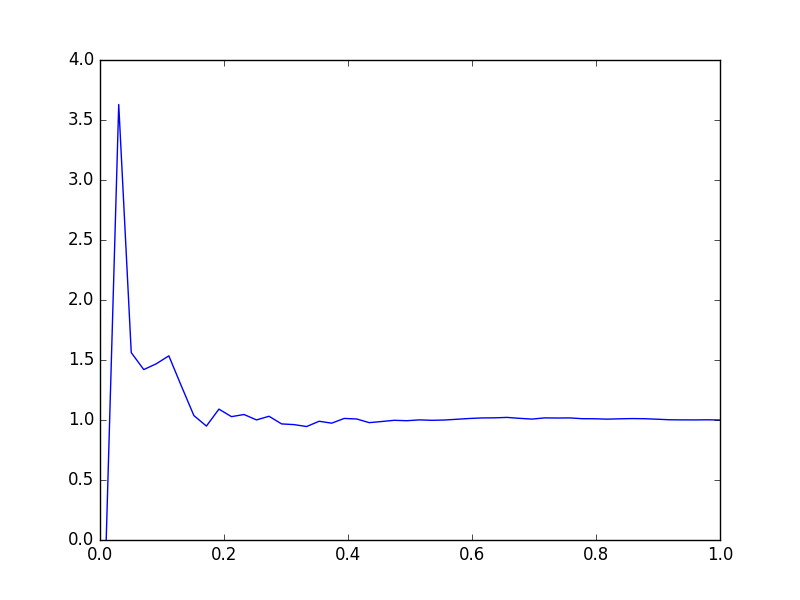
\includegraphics[scale=0.4]{5_b.png}
        \caption{Figure for Problem b (uniform distribution)}
    \end{figure}
    \begin{figure}[H]
        \centering
        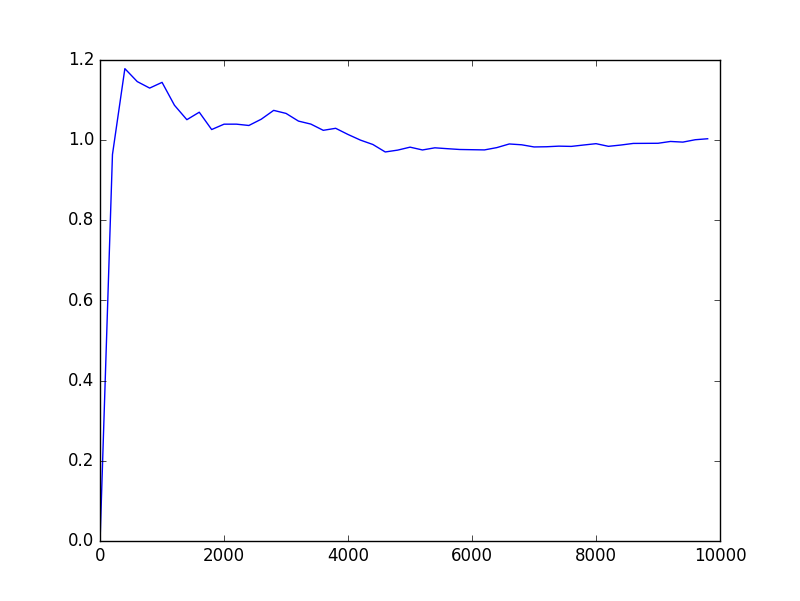
\includegraphics[scale=0.4]{5_c.png}
        \caption{Figure for Problem c (uniform distribution)}
    \end{figure}
    \begin{figure}[H]
        \centering
        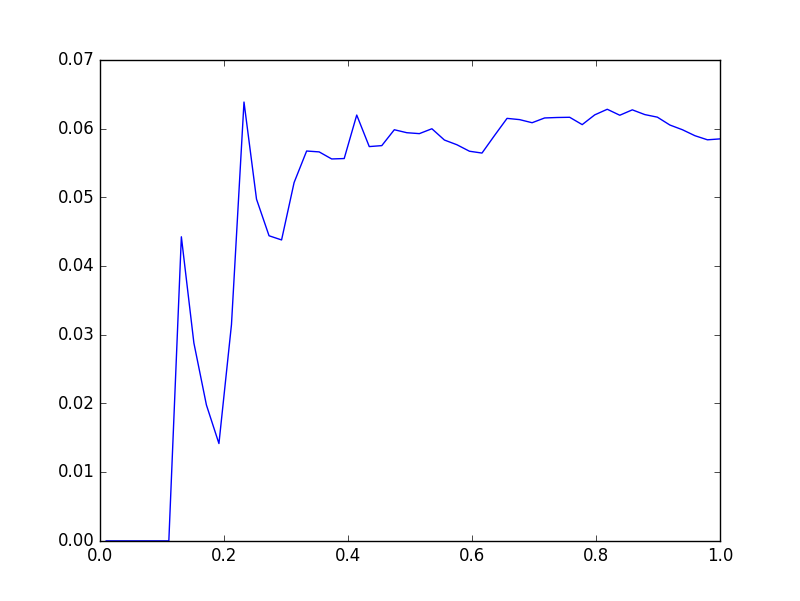
\includegraphics[scale=0.4]{5_d_b.png}
        \caption{Figure for Problem b (gaussian distribution)}
    \end{figure}
    \begin{figure}[H]
        \centering
        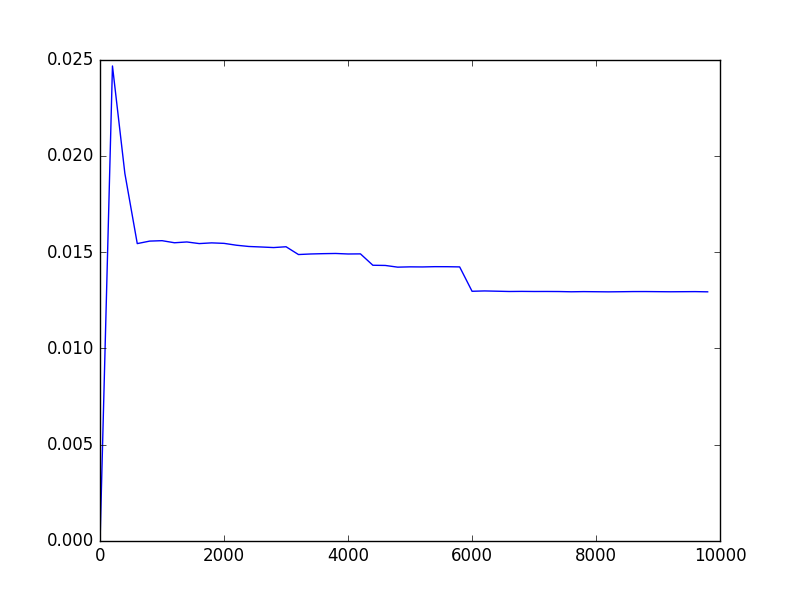
\includegraphics[scale=0.4]{5_d_c.png}
        \caption{Figure for Problem c (gaussian distribution)}
    \end{figure}
    \paragraph{} For uniform distribution two method all goes to $p((0,0,0)) = 1$ when n increase to sufficiently large and its convergence is quick. However, For gaussian distribution, its convergence is much slower than that of uniform distribution.
    \subsection{Code}
    \lstinputlisting[language=Python]{5.py}
    \section{Problem 5}
    \subsection{Result}
    \begin{figure}[H]
        \centering
        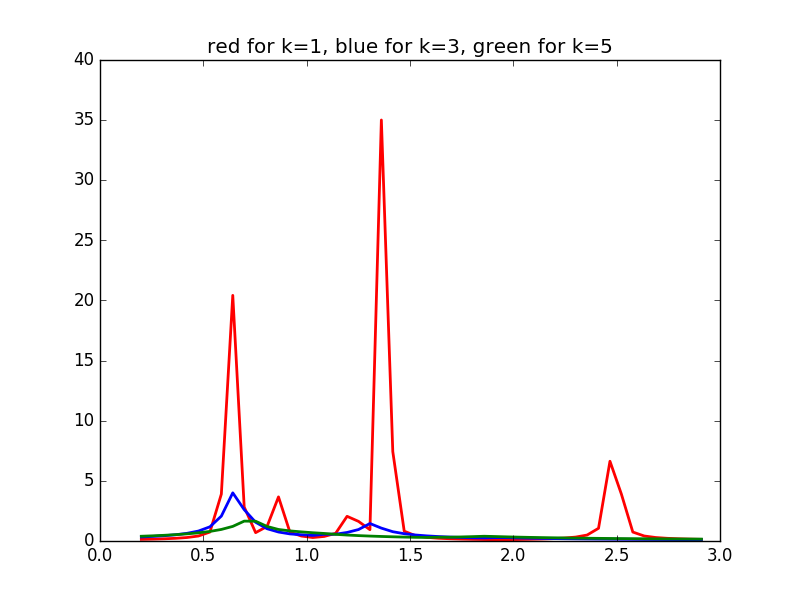
\includegraphics[scale=0.4]{6_a.png}
        \caption{Figure for Problem a}
    \end{figure}
    \begin{figure}[H]
        \centering
        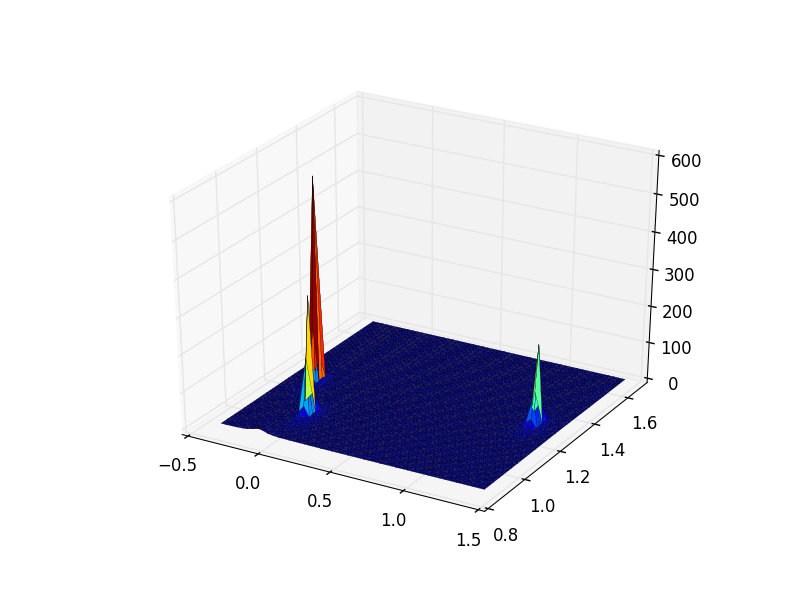
\includegraphics[scale=0.4]{6_b_1.png}
        \caption{Figure for Problem b, k = 1}
    \end{figure}
    \begin{figure}[H]
        \centering
        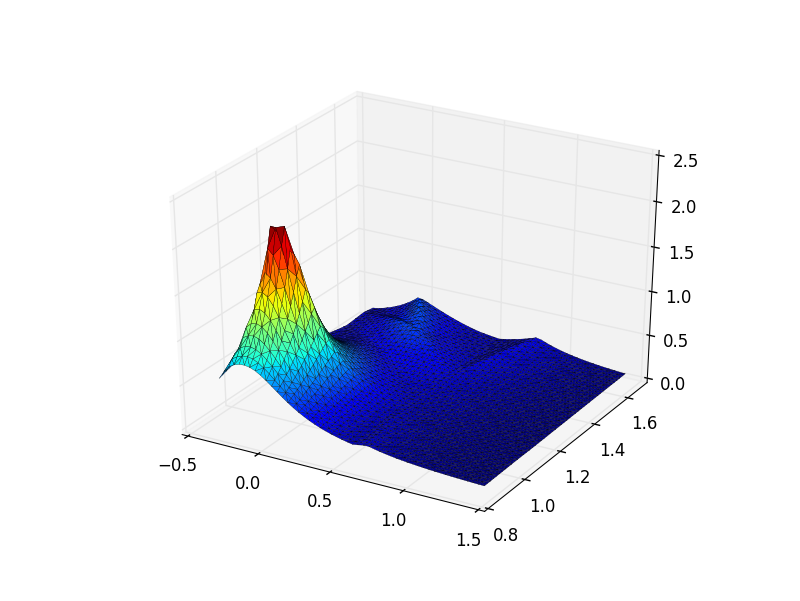
\includegraphics[scale=0.4]{6_b_3.png}
        \caption{Figure for Problem b, k = 3}
    \end{figure}
    \begin{figure}[H]
        \centering
        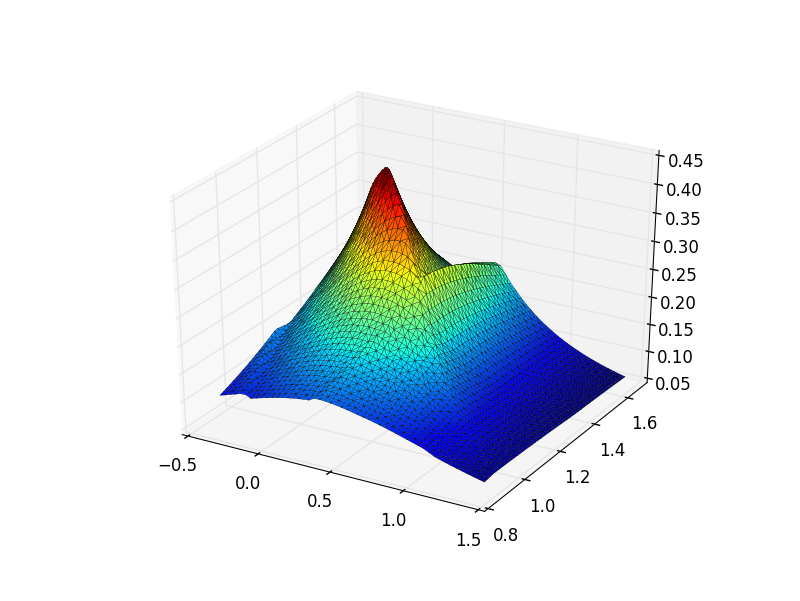
\includegraphics[scale=0.4]{6_b_5.png}
        \caption{Figure for Problem b, k = 5}
    \end{figure}
    \subsection{Code}
    \lstinputlisting[language=Python]{6.py}
\end{document}